\documentclass[aspectratio=169,xcolor=dvipsnames]{beamer}
% 1. Definir el color ANTES de llamar al tema SimplePlus
\usepackage{xcolor}
\definecolor{nyugray}{RGB}{128,128,128}
\usetheme{SimplePlus}
\definecolor{UnalGreen}{RGB}{0,153,51}
\definecolor{StripA}{RGB}{200,60,60}
\definecolor{StripB}{RGB}{60,90,180}
\usepackage[utf8]{inputenc}
\usepackage[T1]{fontenc}
\usepackage[spanish]{babel}
\usepackage{hyperref}
\usepackage{graphicx}
\usepackage{booktabs}
\usepackage{tikz}
\usepackage{pgfplots}
% NOTA: no se declara \pgfplotsset{compat=...} a propósito (ver convenciones del curso)
\usetikzlibrary{positioning, arrows.meta, babel, calc}
\usepackage[skip=5pt]{caption}
\captionsetup{justification=justified, font=small}
\usefonttheme{professionalfonts}


% ----- PLACEHOLDER PARA IMÁGENES EXTERNAS -----
\newcommand{\imgwarning}[2][0.8]{%
	\begin{center}
		\fcolorbox{nyugray}{gray!8}{%
			\parbox[c][3.2cm][c]{#1\textwidth}{\centering\small\textcolor{nyugray}{%
					[\,Insertar imagen: #2\,]}}%
		}
	\end{center}
}

\title{Laboratorio Mecánica y ondas para Biociencias}
\subtitle{Sesión 3: Propagación de errores y Graficación}
\titlegraphic{%
	\vspace*{-0.3cm}%
	\IfFileExists{imagenes/universidad-nacional-de-colombia-sede-bogota-seeklogo.png}{%
		\includegraphics[width=2.2cm]{imagenes/universidad-nacional-de-colombia-sede-bogota-seeklogo.png}%
	}{%
		\IfFileExists{universidad-nacional-de-colombia-sede-bogota-seeklogo.png}{%
			
\includegraphics[width=2.2cm]{universidad-nacional-de-colombia-sede-bogota-seeklogo.png}%
		}{}%
	}%
	\hspace{1.0cm}%
	\IfFileExists{logoMIAI_white.png}{%
		
\includegraphics[width=4.0cm]{logoMIAI_white.png}%
	}{%
		\IfFileExists{imagenes/logoMIAI_white.png}{%
			\includegraphics[width=4.0cm]{imagenes/logoMIAI_white.png}%
		}{}%
	}%
}
\author{Miguel Andrés Perdomo Gutiérrez}
\institute{%
	Auxiliar Docente | M.Sc. en Ciencias -- Física\\
	Universidad Nacional de Colombia -- Sede Bogotá
}
\date{15 de septiembre de 2026}

\begin{document}
	
	% ============================================================
	% SLIDE 1: PORTADA
	% ============================================================
	\begin{frame}
		\titlepage
	\end{frame}
	
	% ============================================================
	% SLIDE 2: AGENDA
	% ============================================================
	\begin{frame}{Agenda de la Sesión}
		\centering
		\begin{tikzpicture}[
			box/.style={rectangle, rounded corners, draw=UnalGreen, thick, fill=UnalGreen!10,
				minimum width=2.3cm, minimum height=1.7cm, align=center, font=\scriptsize},
			arr/.style={-{Latex[length=2mm]}, thick, UnalGreen}
			]
			\node[box] (b1) {Quiz y\\repaso\\\textbf{15 min}};
			\node[box, right=0.35cm of b1] (b2) {Propagación\\de errores\\\textbf{35 min}};
			\node[box, right=0.35cm of b2] (b3) {Graficación\\y linealización\\\textbf{25 min}};
			\node[box, right=0.35cm of b3] (b4) {Tracker\\(demostración)\\\textbf{20 min}};
			\node[box, right=0.35cm of b4] (b5) {Taller 2\\(inicio)\\\textbf{25 min}};
			\draw[arr] (b1) -- (b2);
			\draw[arr] (b2) -- (b3);
			\draw[arr] (b3) -- (b4);
			\draw[arr] (b4) -- (b5);
		\end{tikzpicture}
		
		\vspace{0.5cm}
		\begin{itemize}
			\item Duración total: \textbf{2 horas} (Martes 11:00--13:00, Laboratorio 104, Ed.\ 404).
			\item El Taller 2 se empieza en clase y se termina en casa.
			\item Para la próxima sesión: \textbf{traer portátil} (trabajaremos con Tracker).
		\end{itemize}
	\end{frame}
	
	% ============================================================
	% SLIDE 3: REPASO
	% ============================================================
	\begin{frame}{Repaso: cómo reportamos una medida}
		\begin{exampleblock}{Lo que aprendimos la sesión pasada}
			\centering
			\Large $x = \bar{x} \pm \Delta x$
		\end{exampleblock}
		
		\vspace{0.5cm}
		\begin{center}
			\begin{tikzpicture}[scale=1]
				\draw[thick] (0,0) -- (10,0);
				\fill[UnalGreen!25] (3.6,-0.45) rectangle (6.4,0.45);
				\draw[thick, UnalGreen] (3.6,-0.45) -- (3.6,0.45);
				\draw[thick, UnalGreen] (6.4,-0.45) -- (6.4,0.45);
				\fill[UnalGreen] (5,0) circle (3pt);
				\node[below=8pt] at (5,-0.45) {$\bar{x}$};
				\node[below=8pt] at (3.6,-0.45) {$\bar{x}-\Delta x$};
				\node[below=8pt] at (6.4,-0.45) {$\bar{x}+\Delta x$};
				\node[above=10pt, font=\small] at (5,0.45) {el valor real está en algún lugar de esta franja};
			\end{tikzpicture}
		\end{center}
		
		\vspace{0.6cm}
		\begin{center}
			\textcolor{UnalGreen}{\textbf{Hoy:}} ¿qué pasa con esa franja cuando \emph{operamos}
			con la medida?
		\end{center}
	\end{frame}
	
	% ============================================================
	% SLIDE 4: ¿POR QUÉ PROPAGAR?
	% ============================================================
\begin{frame}{El problema}
	\begin{center}
		\begin{tikzpicture}[
			bx/.style={rectangle, rounded corners, draw, thick,
				minimum width=3.6cm, minimum height=1.2cm,
				align=center, font=\small},
			arr/.style={-{Latex[length=2.5mm]}, very thick, UnalGreen}
			]
			
			% --- Nodos de medición ---
			\node[bx, draw=UnalGreen, fill=UnalGreen!10] (m1)
			{Mido $x = 27.9 \pm 0.1$ cm};
			\node[bx, draw=UnalGreen, fill=UnalGreen!10, below=0.6cm of m1] (m2)
			{Mido $y = 21.6 \pm 0.1$ cm};
			
			% --- Punto medio vertical entre m1 y m2 ---
			\coordinate (mid) at ($(m1.east)!0.5!(m2.east)$);
			
			% --- Nodo resultado, a la derecha del punto medio ---
			\node[bx, draw=StripA, fill=StripA!8, right=2.8cm of mid] (r)
			{Calculo $z = x\cdot y$\\[2pt] $z = 602.6$ cm$^2$};
			
			% --- Flechas: salen al este, van horizontal, giran y entran al oeste ---
			\draw[arr] (m1.east) -- ++(1.0,0) |- (r.west);
			\draw[arr] (m2.east) -- ++(1.0,0) |- (r.west);
		\end{tikzpicture}
	\end{center}
	
	\vspace{0.5cm}
	\begin{alertblock}{La pregunta}
		\centering
		Si $x$ y $y$ tienen incertidumbre, \textbf{¿cuánta incertidumbre tiene $z$?}
	\end{alertblock}
	
	\vspace{0.3cm}
	\begin{center}
		\small Escribir $z = 602.6$ cm$^2$ sin más es \emph{deshonesto}:
		sugiere una precisión que no tenemos.
	\end{center}
\end{frame}
	
	% ============================================================
	% SLIDE 5: SUMAS Y RESTAS
	% ============================================================
	\begin{frame}{Caso 1: sumas y restas}
		\begin{center}
			\begin{tikzpicture}[scale=1]
				% barra 1
				\draw[very thick, UnalGreen] (0,1.6) -- (4,1.6);
				\fill[UnalGreen!30, opacity=0.7] (3.6,1.35) rectangle (4.4,1.85);
				\node[left, font=\small] at (0,1.6) {$x$};
				\node[right, font=\scriptsize] at (4.5,1.6) {$\pm\,\Delta x$};
				
				% barra 2
				\draw[very thick, StripB] (0,0.7) -- (2.6,0.7);
				\fill[StripB!30, opacity=0.7] (2.25,0.45) rectangle (2.95,0.95);
				\node[left, font=\small] at (0,0.7) {$y$};
				\node[right, font=\scriptsize] at (3.05,0.7) {$\pm\,\Delta y$};
				
				% suma
				\draw[very thick, StripA] (0,-0.4) -- (6.6,-0.4);
				\fill[StripA!25, opacity=0.7] (6.05,-0.65) rectangle (7.15,-0.15);
				\node[left, font=\small] at (0,-0.4) {$x+y$};
				\node[right, font=\scriptsize] at (7.25,-0.4) {$\pm\,\Delta(x{+}y)$};
				
				\draw[dashed, gray] (0,1.85) -- (0,-0.9);
			\end{tikzpicture}
		\end{center}
		
		\vspace{0.2cm}
		\begin{exampleblock}{Regla}
			\centering
			\Large $\Delta z = \sqrt{(\Delta x)^2 + (\Delta y)^2}$
			\vspace{0.1cm}
			
			\small (vale igual para $z = x+y$ y para $z = x-y$)
		\end{exampleblock}
		
		\vspace{0.2cm}
		\begin{center}
			\small Se suman las incertidumbres \textbf{absolutas}, en cuadratura.
		\end{center}
	\end{frame}
	
	% ============================================================
	% SLIDE 6: ¿POR QUÉ EN CUADRATURA?
	% ============================================================
	\begin{frame}{¿Por qué en cuadratura y no simplemente sumadas?}
		\begin{center}
			\begin{tikzpicture}[scale=0.95]
				% caso peor
				\node[font=\small\bfseries] at (2,2.6) {Si siempre se sumaran};
				\draw[-{Latex[length=2mm]}, thick, StripA] (0.4,1.9) -- (2.2,1.9);
				\draw[-{Latex[length=2mm]}, thick, StripA] (2.2,1.4) -- (3.6,1.4);
				\node[font=\scriptsize] at (2,0.85) {los dos errores hacia el mismo lado};
				\node[font=\scriptsize, StripA] at (2,0.35) {(muy improbable)};
				
				\draw[gray!50] (5,0.1) -- (5,2.8);
				
				% caso real
				\node[font=\small\bfseries] at (8,2.6) {Lo que realmente pasa};
				\draw[-{Latex[length=2mm]}, thick, StripB] (6.4,1.9) -- (8.2,1.9);
				\draw[-{Latex[length=2mm]}, thick, StripB] (8.2,1.4) -- (7.1,1.4);
				\node[font=\scriptsize] at (8,0.85) {a veces se cancelan parcialmente};
				\node[font=\scriptsize, StripB] at (8,0.35) {(errores independientes)};
			\end{tikzpicture}
		\end{center}
		
		\vspace{0.3cm}
		\begin{block}{}
			\centering
			Sumarlos directamente supone el \textbf{peor caso posible} y sobreestima el error.
			La cuadratura da el resultado \textbf{típico}.
		\end{block}
		
		\vspace{0.2cm}
		\begin{center}
			\small Ejemplo: con $\Delta x = \Delta y = 3$, sumar da $6$;
			la cuadratura da $\sqrt{9+9} \approx 4.2$.
		\end{center}
	\end{frame}
	
	% ============================================================
	% SLIDE 7: PRODUCTOS -- LA IMAGEN
	% ============================================================
	\begin{frame}{Caso 2: productos (¿cuánto crece un área?)}
		\begin{columns}[T]
			\begin{column}{0.55\textwidth}
				\begin{center}
					\begin{tikzpicture}[scale=0.68]
						% franjas
						\fill[StripA!35] (6,0) rectangle (7.1,4);
						\fill[StripB!35] (0,4) rectangle (6,4.8);
						\fill[gray!45] (6,4) rectangle (7.1,4.8);
						
						% rectangulo base
						\fill[UnalGreen!15] (0,0) rectangle (6,4);
						\draw[very thick, UnalGreen] (0,0) rectangle (6,4);
						
						% borde exterior
						\draw[dashed, thick] (0,0) rectangle (7.1,4.8);
						
						% etiquetas
						\node[font=\large] at (3,2) {$A = L\,a$};
						\draw[|-|] (0,-0.5) -- (6,-0.5) node[midway,below,font=\small] {$L$};
						\draw[|-|] (6,-0.5) -- (7.1,-0.5) node[midway,below,font=\scriptsize] {$\Delta L$};
						\draw[|-|] (-0.5,0) -- (-0.5,4) node[midway,left,font=\small] {$a$};
						\draw[|-|] (-0.5,4) -- (-0.5,4.8) node[midway,left,font=\scriptsize] {$\Delta a$};
						
						\node[StripA, font=\scriptsize, right] at (7.3,2) {$a\,\Delta L$};
						\node[StripB, font=\scriptsize] at (3,5.3) {$L\,\Delta a$};
					\end{tikzpicture}
				\end{center}
			\end{column}
			\begin{column}{0.43\textwidth}
				\vspace{0.6cm}
				\small
				Al crecer los dos lados, el área gana \textbf{dos franjas}:
				\[
				\Delta A \approx a\,\Delta L + L\,\Delta a
				\]
				
				\vspace{0.25cm}
				El cuadradito gris de la esquina vale $\Delta L\,\Delta a$: es
				\textbf{despreciable}.
				
				\vspace{0.3cm}
				\textcolor{UnalGreen}{\textbf{Dividiendo entre $A = L\,a$:}}
				\[
				\frac{\Delta A}{A} \approx \frac{\Delta L}{L} + \frac{\Delta a}{a}
				\]
			\end{column}
		\end{columns}
	\end{frame}
	
	% ============================================================
	% SLIDE 8: PRODUCTOS -- LA REGLA
	% ============================================================
	\begin{frame}{Caso 2: productos y cocientes}
		\begin{exampleblock}{Regla}
			\centering
			\Large $\dfrac{\Delta z}{z} = \sqrt{\left(\dfrac{\Delta x}{x}\right)^{2}
				+ \left(\dfrac{\Delta y}{y}\right)^{2}}$
			\vspace{0.1cm}
			
			\small (vale igual para $z = x\cdot y$ y para $z = x/y$)
		\end{exampleblock}
		
		\vspace{0.4cm}
		\begin{alertblock}{La diferencia clave con el caso anterior}
			\centering
			En sumas se combinan las incertidumbres \textbf{absolutas}. \\[3pt]
			En productos se combinan las \textbf{relativas}.
		\end{alertblock}
		
		\vspace{0.3cm}
		\begin{center}
			\small Esta fórmula entrega $\Delta z / z$, un número sin unidades.
			Para obtener $\Delta z$ hay que multiplicar por $z$:
			\[
			\Delta z = z \times \frac{\Delta z}{z}
			\]
		\end{center}
	\end{frame}
	
	% ============================================================
	% SLIDE 9: POTENCIAS -- LA IMAGEN
	% ============================================================
	\begin{frame}{Caso 3: potencias (el cuadrado)}
		\begin{columns}[T]
			\begin{column}{0.5\textwidth}
				\begin{center}
					\begin{tikzpicture}[scale=0.75]
						\fill[StripA!35] (4,0) rectangle (4.9,4);
						\fill[StripA!35] (0,4) rectangle (4,4.9);
						\fill[gray!45] (4,4) rectangle (4.9,4.9);
						
						\fill[UnalGreen!15] (0,0) rectangle (4,4);
						\draw[very thick, UnalGreen] (0,0) rectangle (4,4);
						\draw[dashed, thick] (0,0) rectangle (4.9,4.9);
						
						\node[font=\large] at (2,2) {$t^{2}$};
						\draw[|-|] (0,-0.5) -- (4,-0.5) node[midway,below,font=\small] {$t$};
						\draw[|-|] (4,-0.5) -- (4.9,-0.5) node[midway,below,font=\scriptsize] {$\Delta t$};
						
						\node[StripA, font=\scriptsize, right] at (5.1,2) {$t\,\Delta t$};
						\node[StripA, font=\scriptsize] at (2,5.4) {$t\,\Delta t$};
					\end{tikzpicture}
				\end{center}
			\end{column}
			\begin{column}{0.48\textwidth}
				\vspace{0.6cm}
				\small
				Ahora las dos franjas son \textbf{iguales}: cada una vale $t\,\Delta t$.
				\[
				\Delta(t^{2}) \approx 2\,t\,\Delta t
				\]
				
				\vspace{0.35cm}
				En forma relativa:
				\[
				\frac{\Delta(t^{2})}{t^{2}} = \frac{2t\,\Delta t}{t^{2}} = 2\,\frac{\Delta t}{t}
				\]
				
				\vspace{0.35cm}
				\begin{center}
					\textcolor{UnalGreen}{\textbf{El error relativo se \emph{duplica}.}}
				\end{center}
			\end{column}
		\end{columns}
	\end{frame}
	
	% ============================================================
	% SLIDE 10: RESUMEN DE REGLAS
	% ============================================================
	\begin{frame}{Resumen: las cuatro reglas}
		\begin{center}
			\footnotesize
			\begin{tabular}{@{}llc@{}}
				\toprule
				\textbf{Operación} & \textbf{Cómo se propaga} & \textbf{Fórmula} \\
				\midrule
				$z = x \pm y$   & absolutos, en cuadratura
				& $\Delta z = \sqrt{(\Delta x)^2 + (\Delta y)^2}$ \\[5pt]
				
				$z = x\cdot y$ \ ó \ $x/y$ & relativos, en cuadratura
				& $\dfrac{\Delta z}{z} = \sqrt{\left(\dfrac{\Delta x}{x}\right)^2
					+ \left(\dfrac{\Delta y}{y}\right)^2}$ \\[9pt]
				
				$z = c\cdot x$ \ ($c$ constante) & el absoluto se multiplica por $c$
				& $\Delta z = c\,\Delta x$ \\[5pt]
				
				$z = x^{n}$ & el relativo se multiplica por $n$
				& $\dfrac{\Delta z}{z} = |n|\,\dfrac{\Delta x}{x}$ \\
				\bottomrule
			\end{tabular}
		\end{center}
		
		\vspace{0.4cm}
		\begin{center}
			\small \textcolor{UnalGreen}{\textbf{La pregunta que hay que hacerse siempre:}}
			¿esta operación es una \emph{suma} o un \emph{producto}?
			De eso depende si uso absolutos o relativos.
		\end{center}
	\end{frame}
	
	
	% ============================================================
	% SLIDE 12: LOS DATOS (GRAFICACIÓN)
	% ============================================================
	\begin{frame}{Los datos: volumen de un gas vs.\ temperatura}
		\begin{center}
			\footnotesize
			\begin{tabular}{lccccccccc}
				\toprule
				$T$ ($^\circ$C) & 62.3 & 68.6 & 81.4 & 87.4 & 98.6 & 104.5 & 116.9 & 121.2 & 135.0 \\
				\midrule
				$V$ (cm$^3$) & 27073 & 28492 & 29300 & 29200 & 30849 & 31500 & 32100 & 32000 & 33500 \\
				\bottomrule
			\end{tabular}
		\end{center}
		
		\vspace{0.4cm}
		\begin{center}
			\small
			Los mismos datos se graficaron de tres maneras distintas.
			Observen cada panel y decidan cuál usarían en un informe y por qué.
		\end{center}
	\end{frame}
	
	% ============================================================
	% SLIDE 13: PANEL (a)
	% ============================================================
	\begin{frame}{Panel (a)}
		\begin{center}
			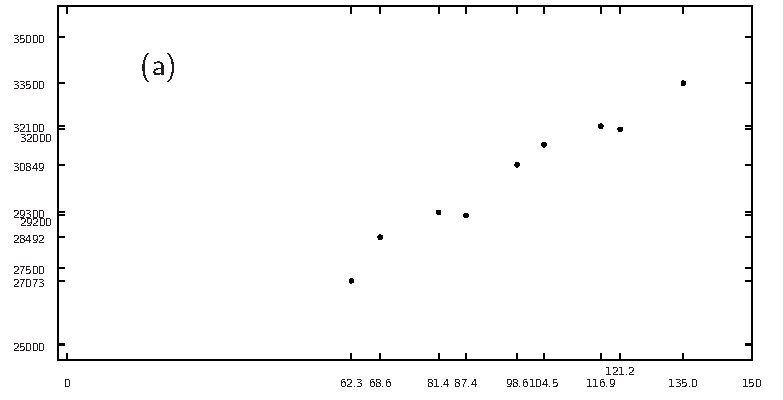
\includegraphics[width=\textwidth,height=0.78\textheight,keepaspectratio]{figura1.pdf}
		\end{center}
	\end{frame}
	
	% ============================================================
	% SLIDE 14: PANELES (b) Y (c)
	% ============================================================
	\begin{frame}{Paneles (b) y (c)}
		\begin{center}
			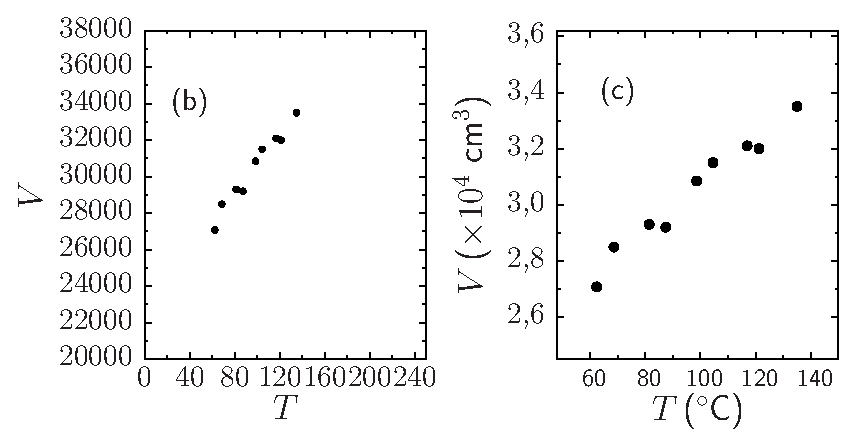
\includegraphics[width=\textwidth,height=0.78\textheight,keepaspectratio]{figura2.pdf}
		\end{center}
	\end{frame}
	
	% ============================================================
	% SLIDE 15: CHECKLIST DE UNA BUENA GRÁFICA
	% ============================================================
	\begin{frame}{Lista de verificación para sus gráficas}
		\begin{enumerate}
			\setlength{\itemsep}{7pt}
			\item Ejes rotulados con su \textbf{magnitud} y su \textbf{unidad}.
			\item Factor común extraído al rótulo: escribir 3.0 con el eje en
			$\times 10^4$, en vez de 30000.
			\item Rango ajustado: los datos deben ocupar buena parte del área.
			\item Marcas del eje en \textbf{valores redondos} y regularmente
			espaciados --- nunca sobre los datos mismos.
			\item Puntos visibles, con sus \textbf{barras de error}.
		\end{enumerate}
		
		\vspace{0.5cm}
		\begin{center}
			\small Esto aplica a todas las gráficas del semestre:
			talleres, bitácoras e informes.
		\end{center}
	\end{frame}
	
	% ============================================================
	% SLIDE 16: LINEALIZACIÓN (GALILEO)
	% ============================================================
	\begin{frame}{Linealizar: la idea de Galileo}
		\begin{columns}[T]
			\begin{column}{0.5\textwidth}
				\small
				Si
				\[
				h = \tfrac{1}{2}g\,t^2
				\]
				entonces al graficar $h$ contra $t^2$ (\textbf{no} contra $t$) se
				obtiene una \textbf{recta} de pendiente $m = g/2$.
				
				\vspace{0.25cm}
				\[
				g_{\text{exp}} = 2 \times m
				\]
				
				\vspace{0.3cm}
				\textcolor{UnalGreen}{\textbf{¿Por qué molestarse?}}
				\begin{itemize}\small
					\item De una curva no se lee una constante.
					\item De una recta, sí: es su pendiente.
				\end{itemize}
			\end{column}
			\begin{column}{0.5\textwidth}
				\begin{center}
					\begin{tikzpicture}
						\begin{axis}[width=6.0cm, height=4.6cm,
							xlabel={$t^2$ (s$^2$)}, ylabel={$h$ (m)},
							xmin=0, xmax=2.2, ymin=0, ymax=11,
							xtick={0,0.5,1,1.5,2}, ytick={0,2,4,6,8,10},
							grid=both, grid style={gray!30, thin}]
							\addplot[only marks, mark=*, mark size=1.8pt, UnalGreen]
							coordinates {(0.408,2) (0.816,4) (1.224,6) (1.633,8) (2.041,10)};
							\addplot[domain=0:2.2, samples=2, thick, red!70!black, dashed] {4.9*x};
						\end{axis}
					\end{tikzpicture}
				\end{center}
				\vspace{-0.2cm}
				\begin{center}
					\scriptsize Pendiente $m \approx 4.9 \Rightarrow g \approx 9.8$ m/s$^2$
				\end{center}
			\end{column}
		\end{columns}
	\end{frame}
	
	% ============================================================
	% SLIDE 17: TRACKER -- QUÉ ES
	% ============================================================
	\begin{frame}{Tracker: análisis de video}
		\begin{block}{¿Qué es?}
			Un programa \textbf{gratuito y de código abierto} que permite extraer
			datos de posición y tiempo a partir de un video, cuadro por cuadro.
		\end{block}
		
		\vspace{0.4cm}
		\begin{center}
			\begin{tikzpicture}[
				bx/.style={rectangle, rounded corners, draw=UnalGreen, thick,
					fill=UnalGreen!10, minimum width=2.7cm, minimum height=1.2cm,
					align=center, font=\scriptsize},
				arr/.style={-{Latex[length=2mm]}, thick, UnalGreen}
				]
				\node[bx] (t1) {Grabar el video\\del movimiento};
				\node[bx, right=0.4cm of t1] (t2) {Marcar el objeto\\cuadro por cuadro};
				\node[bx, right=0.4cm of t2] (t3) {Obtener tabla\\de $x$, $y$, $t$};
				\node[bx, right=0.4cm of t3] (t4) {Graficar\\y analizar};
				\draw[arr] (t1) -- (t2);
				\draw[arr] (t2) -- (t3);
				\draw[arr] (t3) -- (t4);
			\end{tikzpicture}
		\end{center}
		
		\vspace{0.5cm}
		\begin{center}
			\small Descarga y documentación: \\[3pt]
			\url{https://opensourcephysics.github.io/tracker-website/}
		\end{center}
	\end{frame}
	
	% ============================================================
	% SLIDE 19: PARA LA PRÓXIMA
	% ============================================================
	\begin{frame}{Para la próxima sesión}
		\begin{alertblock}{Traer portátil}
			\centering
			Con \textbf{Tracker ya instalado}. Descárguenlo desde:
			\vspace{0.2cm}
			
			\url{https://opensourcephysics.github.io/tracker-website/}
		\end{alertblock}
		
		\vspace{0.4cm}
		\begin{itemize}
			\setlength{\itemsep}{6pt}
			\item Basta con \textbf{un portátil por grupo}.
			\item Instálenlo \textbf{antes} de llegar: la descarga en el laboratorio
			toma tiempo.
			\item Si tienen problemas con la instalación, escríbanme con anticipación.
		\end{itemize}
		
		\vspace{0.4cm}
		\begin{center}
			\small La Práctica 1 (Plano Inclinado) es el \textbf{22 de septiembre}.
		\end{center}
	\end{frame}
	
	% ============================================================
	% SLIDE 20: TALLER 2
	% ============================================================
	\begin{frame}{Taller 2: manos a la obra}
		\begin{block}{Lo que van a hacer}
			\begin{enumerate}
				\item \textbf{Parte A:} medir una hoja de papel y propagar la
				incertidumbre al área (producto).
				\item \textbf{Parte B:} graficar $h$ contra $t^2$ con barras de error
				en ambos ejes, trazar la recta y obtener $g$.
			\end{enumerate}
		\end{block}
		
		\vspace{0.4cm}
		\begin{itemize}
			\item Es \textbf{individual}. Se empieza en clase y se termina en casa.
			\item Necesitan regla, papel milimetrado y calculadora.
		\end{itemize}
		
		\vspace{0.5cm}
		\begin{center}
			\large \textcolor{UnalGreen}{\textbf{Todo lo de hoy, aplicado a sus propios cálculos.}}
		\end{center}
	\end{frame}
	
	% ============================================================
	% SLIDE 21: CIERRE
	% ============================================================
	\begin{frame}{¿Preguntas o Comentarios?}
		\begin{center}
			\vspace{0.5cm}
			\Large Nos vemos la próxima sesión.
			
			\vspace{0.8cm}
			\normalsize
			mperdomog@unal.edu.co
			
			\vspace{0.2cm}
			Laboratorio 104 -- Edificio 404
		\end{center}
	\end{frame}
	
\end{document}